\section{RAS\_\-stack\_\-t Class Reference}
\label{classRAS__stack__t}\index{RAS\_\-stack\_\-t@{RAS\_\-stack\_\-t}}
Inheritance diagram for RAS\_\-stack\_\-t:\nopagebreak
\begin{figure}[H]
\begin{center}
\leavevmode
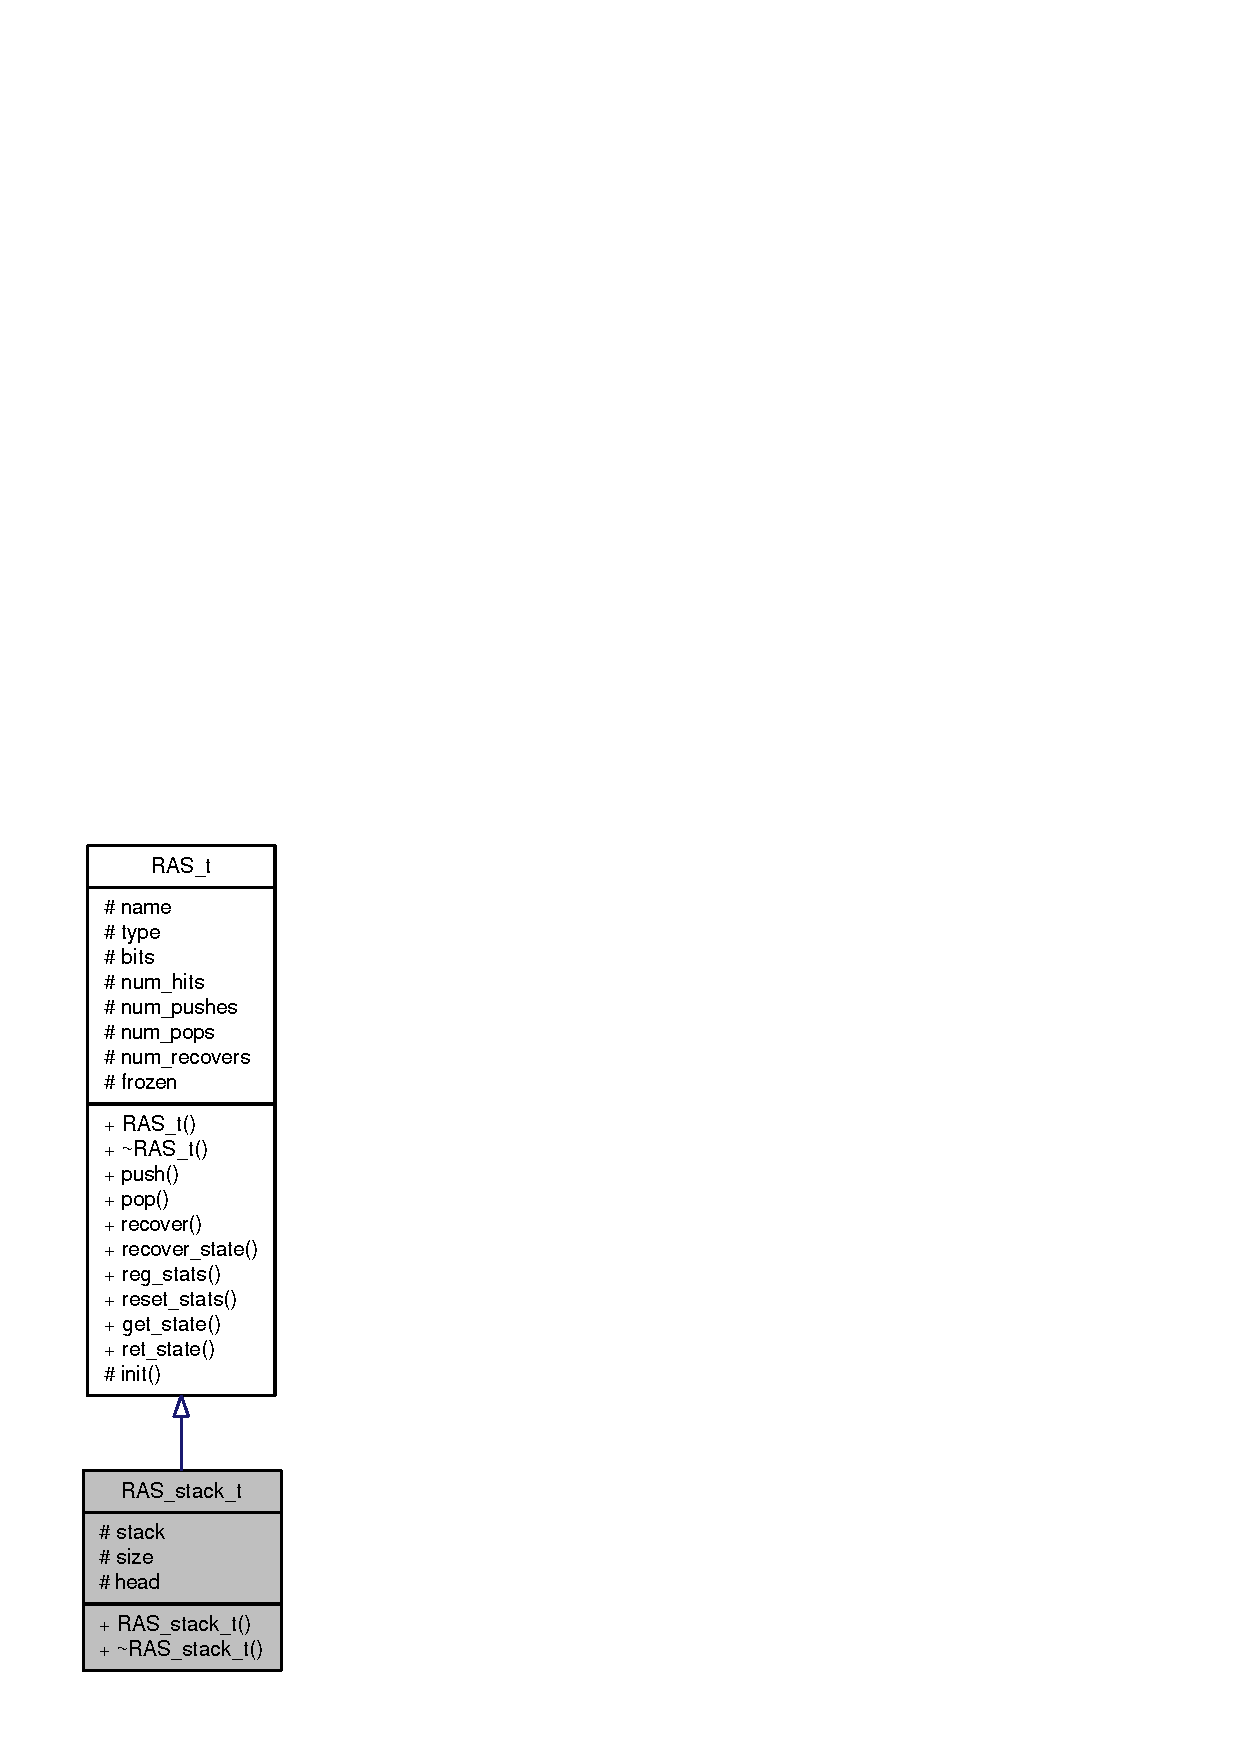
\includegraphics[height=400pt]{classRAS__stack__t__inherit__graph}
\end{center}
\end{figure}
Collaboration diagram for RAS\_\-stack\_\-t:\nopagebreak
\begin{figure}[H]
\begin{center}
\leavevmode
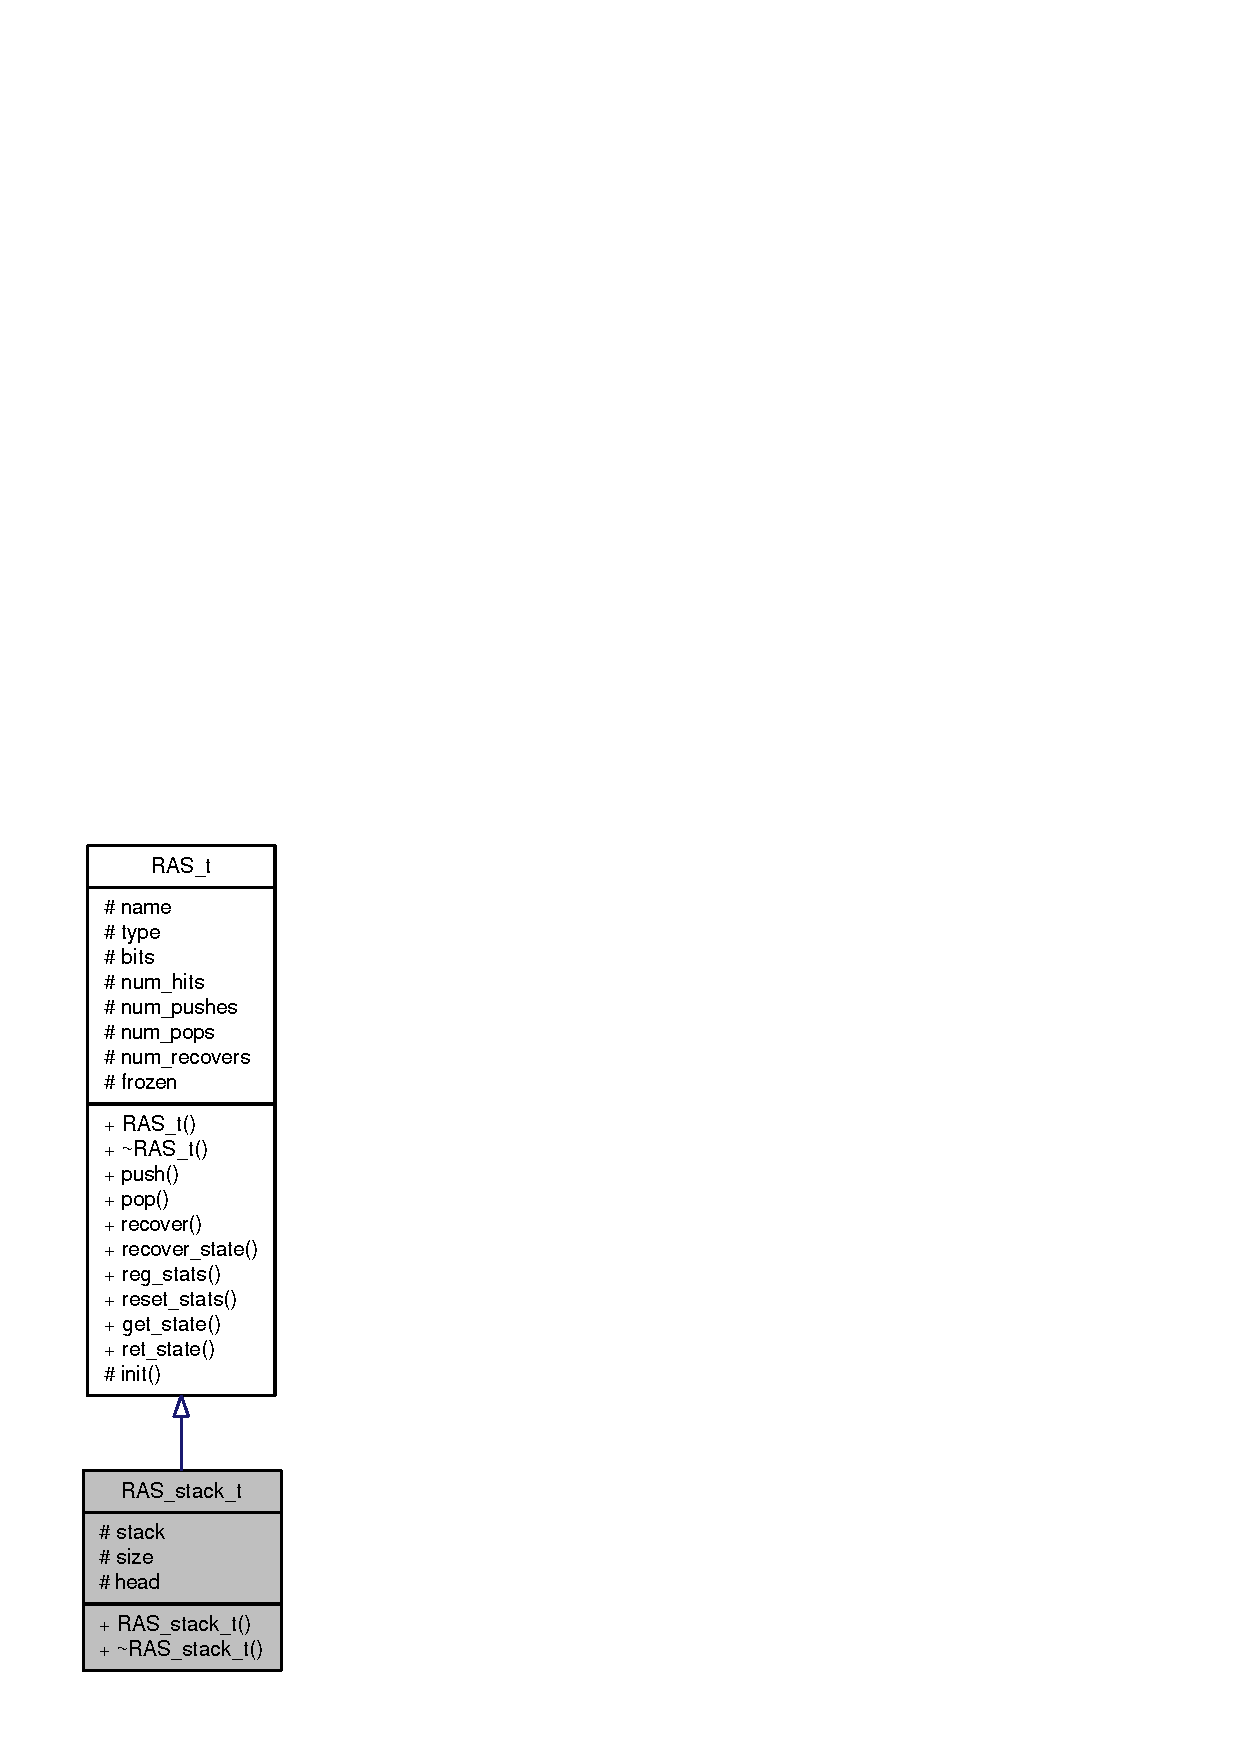
\includegraphics[height=400pt]{classRAS__stack__t__coll__graph}
\end{center}
\end{figure}
\subsection*{Classes}
\begin{CompactItemize}
\item 
class {\bf RAS\_\-stack\_\-chkpt\_\-t}
\end{CompactItemize}
\subsection*{Public Member Functions}
\begin{CompactItemize}
\item 
{\bf RAS\_\-stack\_\-t} (char $\ast$const arg\_\-name, const int arg\_\-num\_\-entries)
\item 
{\bf $\sim$RAS\_\-stack\_\-t} ()
\end{CompactItemize}
\subsection*{Protected Attributes}
\begin{CompactItemize}
\item 
{\bf md\_\-addr\_\-t} $\ast$ {\bf stack}
\item 
int {\bf size}
\item 
int {\bf head}
\end{CompactItemize}


\subsection{Detailed Description}


Definition at line 18 of file ras-stack.cpp.

\subsection{Constructor \& Destructor Documentation}
\index{RAS\_\-stack\_\-t@{RAS\_\-stack\_\-t}!RAS\_\-stack\_\-t@{RAS\_\-stack\_\-t}}
\index{RAS\_\-stack\_\-t@{RAS\_\-stack\_\-t}!RAS_stack_t@{RAS\_\-stack\_\-t}}
\subsubsection[{RAS\_\-stack\_\-t}]{\setlength{\rightskip}{0pt plus 5cm}RAS\_\-stack\_\-t::RAS\_\-stack\_\-t (char $\ast$const  {\em arg\_\-name}, \/  const int {\em arg\_\-num\_\-entries})\hspace{0.3cm}{\tt  [inline]}}\label{classRAS__stack__t_659d357a08ac30f13bf83993dd61bc1b}




Definition at line 35 of file ras-stack.cpp.

References RAS\_\-t::bits, fatal(), head, RAS\_\-t::init(), RAS\_\-t::name, size, stack, and RAS\_\-t::type.\index{RAS\_\-stack\_\-t@{RAS\_\-stack\_\-t}!$\sim$RAS\_\-stack\_\-t@{$\sim$RAS\_\-stack\_\-t}}
\index{$\sim$RAS\_\-stack\_\-t@{$\sim$RAS\_\-stack\_\-t}!RAS_stack_t@{RAS\_\-stack\_\-t}}
\subsubsection[{$\sim$RAS\_\-stack\_\-t}]{\setlength{\rightskip}{0pt plus 5cm}RAS\_\-stack\_\-t::$\sim$RAS\_\-stack\_\-t ()\hspace{0.3cm}{\tt  [inline]}}\label{classRAS__stack__t_567f7b63162e12c15c783cb999b5e9c1}




Definition at line 57 of file ras-stack.cpp.

References RAS\_\-t::name, stack, and RAS\_\-t::type.

\subsection{Member Data Documentation}
\index{RAS\_\-stack\_\-t@{RAS\_\-stack\_\-t}!head@{head}}
\index{head@{head}!RAS_stack_t@{RAS\_\-stack\_\-t}}
\subsubsection[{head}]{\setlength{\rightskip}{0pt plus 5cm}int {\bf RAS\_\-stack\_\-t::head}\hspace{0.3cm}{\tt  [protected]}}\label{classRAS__stack__t_d43a39ae16eb6a362089c6eb00a354fc}




Definition at line 30 of file ras-stack.cpp.

Referenced by RAS\_\-stack\_\-t().\index{RAS\_\-stack\_\-t@{RAS\_\-stack\_\-t}!size@{size}}
\index{size@{size}!RAS_stack_t@{RAS\_\-stack\_\-t}}
\subsubsection[{size}]{\setlength{\rightskip}{0pt plus 5cm}int {\bf RAS\_\-stack\_\-t::size}\hspace{0.3cm}{\tt  [protected]}}\label{classRAS__stack__t_68c8edf975a2ca73dda9087563cc2ee6}




Definition at line 29 of file ras-stack.cpp.

Referenced by RAS\_\-stack\_\-t().\index{RAS\_\-stack\_\-t@{RAS\_\-stack\_\-t}!stack@{stack}}
\index{stack@{stack}!RAS_stack_t@{RAS\_\-stack\_\-t}}
\subsubsection[{stack}]{\setlength{\rightskip}{0pt plus 5cm}{\bf md\_\-addr\_\-t}$\ast$ {\bf RAS\_\-stack\_\-t::stack}\hspace{0.3cm}{\tt  [protected]}}\label{classRAS__stack__t_41dce029c72eb86f0f7725260d108b56}




Definition at line 28 of file ras-stack.cpp.

Referenced by RAS\_\-stack\_\-t(), and $\sim$RAS\_\-stack\_\-t().

The documentation for this class was generated from the following file:\begin{CompactItemize}
\item 
{\bf ras-stack.cpp}\end{CompactItemize}
